\documentclass[lettersize,journal]{IEEEtran}
\usepackage{amsmath,amsfonts}
\usepackage{algorithmic}
\usepackage{algorithm}
\usepackage{array}
\usepackage[caption=false,font=normalsize,labelfont=sf,textfont=sf]{subfig}
\usepackage{textcomp}
\usepackage{stfloats}
\usepackage{url}
\usepackage{verbatim}
\usepackage{graphicx}
\usepackage{cite}
\hyphenation{op-tical net-works semi-conduc-tor IEEE-Xplore}
% updated with editorial comments 8/9/2021

\usepackage{caption}
\usepackage{subcaption}
\usepackage{hyperref}
\hypersetup{
    colorlinks=true,
    linkcolor=blue,
    citecolor=blue,
    filecolor=magenta,      
    urlcolor=cyan,
    pdftitle={Overleaf Example},
    pdfpagemode=FullScreen,
    }

\begin{document}

\title{Significance of Image Preprocessing using Colour Filters for Automatic Annotation of Segmentation Models, A Review}

\author{Ashwin Rajesh
% <-this % stops a space
\thanks{This paper was produced by the IEEE Publication Technology Group. They are in Piscataway, NJ.}% <-this % stops a space
\thanks{Manuscript received April 19, 2021; revised August 16, 2021.}}

% The paper headers
\markboth{Journal of \LaTeX\ Class Files,~Vol.~14, No.~8, August~2021}%
{Shell \MakeLowercase{\textit{et al.}}: A Sample Article Using IEEEtran.cls for IEEE Journals}

\IEEEpubid{0000--0000/00\$00.00~\copyright~2021 IEEE}
% Remember, if you use this you must call \IEEEpubidadjcol in the second
% column for its text to clear the IEEEpubid mark.

\maketitle

\begin{abstract}
        This document describes the most common article elements and how to use the IEEEtran class with \LaTeX \ to produce files that are suitable for submission to the IEEE.  IEEEtran can produce conference, journal, and technical note (correspondence) papers with a suitable choice of class options. 
\end{abstract}

% \begin{IEEEkeywords}
% Article submission, IEEE, IEEEtran, journal, \LaTeX, paper, template, typesetting.
% \end{IEEEkeywords}

\section{Introduction}
\IEEEPARstart{W}{ildfires} pose a significant threat to humans, wildlife and the
environment alike. Left unchecked, A wildfire can spread rapidly causing
large scale destruction to forests \& infrastructure, as well as
releasing large amounts of pollutants into the atmosphere.

Studies have uncovered very strong associations of wildfire smoke with cardiovascular mortality, asthma hospitalisation and further susceptibility to cardiopulmonary effects in elderly adults.
The risk of premature death and respiratory morbidity in the general population are also increased due to wildfilre smoke \cite{wildfirehealth}.
Furthermore, ambient air pollution caused by wildfire smoke has been studied to have adverse affects on children, as a result of their developing lungs and inferior nasal deposition \cite{wildfirechildren}.
Breathing in wildfire smoke can cause chest pain and tightness, trouble breathing, diziness and other symptoms in children \cite{wildfirefactsheet}.

Wildfires have been consuming increasingly large areas of forest globally in recent years, causing vast amounts of damage to the environment in the form of water \& air pollution, climate change and destruction of flora and fauna.
Sediment exports in water bodies reportedly may increase by up to 1459 times the unburned amount, drastically degrading water quality in the affected areas. \cite{wildfirewater}.
Emissions of airborne particulate matter from wildfires can significant cause significant disruptions to air pollution mitigation targets set by legislation. \cite{wildfireair} shows that in high-fire seasons, pollution levels can reach dangerous levels despite aggressive reduction of anthropogenic emissions.
An estimated 97000 km\textsuperscript{2} of vegetation was burned in the 2019-2020 Australian bushfires, causing devastating damage to wildlife habitat, with many belonging to species listed at threatened to extinction \cite{wildfireveg}.

Evidently, It has become increasingly crucial to detect wildfires as early as possible to minimize damage to humans and the environment. Current methods of wildfire detection involve three main approaches:
\begin{enumerate}
\item{Terrestrial sensor nodes, which may be placed at fire-prone locations to detect wildfires through environmental readings.}
\item{UAVs can be employed to scan large forest areas and inaccessible terrain.}
\item{Satellite based systems can cover vast areas of land and determine the extent and direction of wildfires.}
\end{enumerate}

Despite the various classifications of technologies within wildfire
detection, advancements in computer vision object detection has spurred
use in terrestrial, aerial as well as satellite systems. \cite{satellite}
explores the feasibility of space-borne fire detection using onboard
computer vision to rapidly generate alerts. The traditional method of
downloading image data from satellites has too much latency for
time-sensitive applications such as fire detection. By examining
performance of hardware accelerators for edge computing such as Nvidia
Jetson and Movidius Myriad 2, the report found that AI inference
on-board the satellite is possible in terms of performance as well as
power consumption, allowing for low latency detection of wildfires.
\cite{uavai} details methods to optimise Deep Learning to deal with UAV
limitations such as image degredation, small fire size \& background
complexity. By combining EfficientNet-B5, vision transformers and
EfficientSeg convolutional model, an accuracy of 85.12\% was obtained,
outperforming many state-of-the-art models. \cite{wsnyolo} proposes a low
cost WSN fire detection approach based on YOLO object detection models.
The system, named SDFS was trained on a dataset of 26,520 images and
achieved a high precision rate of 97.1\% for smoke and fire
classification.
\IEEEpubidadjcol

Due to the importance of computer vision based object detection in
wildfire detection, it is imperative that they are as accurate as
possible. There are many different techniques to improve the performance
of neural networks. Transfer learning is the process of using a model
that has been pre-trained on a large dataset and further training and
fine tuning it to a specific task. \cite{transferlearning} studies the
impact of transfer learning on classification by comparing six differnet
pre-trained architectures. The models were trained using an open access
dataset of 3886 images and found that all six architectures were able to
achieve a testing accuracy of above 90\% despite a relatively small
training dataset. Augmenting data with synthetically generated samples
investigated by \cite{augment} found that inserting data-space
transformations such as warped images provided improved performance and
reduced overfitting. \cite{prepfire} proposed an image pre-processing
pipeline using advanced techniques such as HSV filters and corner
detection to assist models with classification by eliminating unwanted
noise in images. This method has observed to improve fire detection
accuracy by 5.5\% and smoke detection by 6\% in object detection models.
Models which allow for finer, more detailed inference called image segmentation models are also improving.
These models combine fully convolutional networks with skip architecture to achieve accurate pixel-wise inference of objects \cite{segmentation}.

% ISSUES
% come around to edge computing CV problem here
\subsection{Existing Issues}
Recent computer vision models are remarkably accurate at wildfire classification. However, they fail to provide any further insights into the state of the wildfire excluding a binary classification. For instance, Knowing the exact shape can be vital information for fire front tracking, which in turn provides valuable insight on which areas the wildfire could spread to. Traditional object detection models fail to capture to the precise dimensions of the fire, as the shape of a fire front is too intricate to be represented by a bounding box. In addition, existing methods of wildfire detection are often performed in remote terrestrial regions, aerially or from space, which will limit the computational power available for running neural networks. Extensively trained Deep neural networks suffer from slower inference, while lightweight shallow networks sacrifice accuracy for prediction speed improvements, therefore limiting the effectiveness of computer vision models in wildfire detection application. Furthermore, existing research regarding methods to track the spread of wildfires is rudimentary. Segmetation models have been under-utilized in wildfire detection applications due to the lack of annotated training data. 

% ADDRESSING THE PROBLEM

This report aims to review methods to enable the tracking and monitoring of wildfires, with a focus on incorporating image segmentation models. Fire detection is currentl carried out through a variety of mediums, such as terrestrial sensor nodes, UAV scanning and satellite based approaches. Observing the literature, it is apparent that computer vision plays a significant role in all systems, Making it important to maximise their efficiency. To this end, methods to automatically annotate image segmentation datasets, including a novel HSV filtering based approach, are examined to determine the ideal way to obtain training data for segmentation models. 

Specifically, auto annotation using an existing object detection model combined with a prompt based segmentation model such as SAM is compared with creating fire masks using HSV colour filtering. Models are trained with the resulting datasets with identical hyperparameters and training time.

This paper contributes firstly a colour filtering based auto annotation approach which can be used to segment objects with predictable colour characteristics. Secondly, a comparison of automatic annotation methods for fire detection is provided.

% This report aims to explore different methods employed in improving the
% performance and efficiency of wildfire detection systems, with a focus
% on computer vision based fire detection using Convolutional Neural
% Networks (CNNs). Fire and smoke detection is carried out through a variety of
% mediums, such as terrestrial sensor nodes, UAV scanning and satellite
% based approaches. Observing the literature, it is apparent that computer
% vision plays a significant role in all systems, Making it important to
% maximise their efficiency and accuracy. Furthermore, it is important to
% optimise such systems to run on low-powered edge computing devices,
% which are currently used to detect wildfires. To this end, a multitude
% of image preprocessing filters relevant to smoke detection were explored. 
% A pipeline of processing that involves Dark Channel Prior in combination with smoke edge detection with Sobel kernels is proposed and benchmarked in this report. 
% The proposed dark channel prior + edge detection algorithm
% aims to improve on existing methods of smoke preprocessing using DCP
% detailed in \cite{prepfire}. Specifically, false positives due to high
% light intensity artifacts in the image such as the sky are significantly
% mitigated, thanks to edge detection filters revealing characteristics
% that are unique to smoke.

% The benchmarks are carried out on a Raspberry Pi 4B, to
% similate low-powered edge computing hardware that is consistently used
% in terrestrial, UAV and satellite systems. Large deep-learning networks
% are unviable on these systems due to the high computational intensity,
% while models with reduced parameters are more efficient but suffer from
% less accurate inference. The preprocessing pipeline aims to improve the
% accuracy of lightweight models by highlighting important features in
% fire and smoke, while reducing unwanted noise in the image.
% To this end, a YOLOv8 nano model is trained on an open source Wildfire Smoke Detection dataset \cite{yolov8}.
% This model is compared with another model that has been trained on the exact same dataset, but with the smoke enhancing preprocessing pipeline stated above.

%Furthermore, an improved system for early smoke detection is
%investigated. 
% This paper contributes a benchmark of different pre-processing filters
%and algorithms to uncover insights on an ideal pipeline for wildfire
%detection, using metrics such as speed, power consumption and model
%accuracy.

\section{Literature Review}

\subsection{Approaches to Fire Detection}


\begin{figure}
        \centering
        \includegraphics[width=2.5in]{sensornode.png}
        \caption{Basic operation of WSNs. Images sourced from Creative Commons,
        following the guidelines on Attribution 3.0 Unported, CC By 3.0}
\end{figure}

\begin{figure}
        \centering
        \includegraphics[width=2.5in]{wildfire_satellite.png}
        \caption{Satellite Based Wildfire Detection}
\end{figure}

Edge computing sensor nodes can be placed at high risk locations that
can monitor temperature, humidity and other characteristics of air in
the surrounding area. These systems generally use a microcontroller to
operate sensors, relying on solar cells for long-term power. By setting
up multiple such nodes in different areas forming a Wireless Sensor
Network (WSN), the collected sensor data may then be analyzed to
determine the locations of fire events \cite{MohapatraAnkita2022EWDT}.
More advance methods of data classification with the use of artificial
neural networks boast a high accuracy of \textgreater82\% with multiple
sensors \cite{wsnfire}. The low cost of WSN systems has made it an
increasingly popular choice for real-time monitoring of forest fires.
However, sensor nodes fail to be viable in some situations. Establishing
wireless communications for a WSN can prove challenging in rural or
untamed areas such as forests \cite{wsnyolo}. The sensor nodes may also
be prone to damage from the wildfire, needing to be replaced in order to
continue using the system.

UAVs have seen extensive research for this application, as they provide
valuable visual data which can be employed to carry out search and
rescue operations, save forest resources, help firefighters navigate
efficiently amoung numerous other enhancements. Rather than sending
ground crews to monitor hazardous environments, UAVs can drastically
reduce the risk to firefighting crews by remotely scanning large amounts
of dangerous forest area. However UAVs tend to perform poorly in harsh
weather conditions, have limited flight time and require a human
operator to have a visual line of sight \cite{uav}. These factors
combined with expensive operation costs severly limit the effectiveness
of UAVs in many circumstances.

Satellite-based fire detection can potentially offer significant
advantages over traditional methods due to the vast areas they can
monitor. The benefits and limitations of these systems largely depend on
the satellite's orbit. Satellites in Sun-Synchronous Orbit (SSO) provide
high spatial resolution but revisit the same location only after several
days, resulting in low temporal resolution. This delay makes SSO
satellites less effective for real-time wildfire detection
\cite{satellite}. In contrast, Geostationary Earth Orbit (GEO) satellites
remain fixed over the same region, as their orbital period matches
Earth's rotation. Equipped with multispectral imaging sensors, GEO
satellites provide continuous monitoring, making them ideal for
detecting and tracking fires in real time.

\subsection{Existing Fire Tracking Methods}
Recent studies indicate experimentation with data-driven approaches to wildfire tracking. \cite{wildfiretrackuavswarm} proposes a UAV swarm utilized as a sensor network to keep track of the border region of a wildfire. The UAV team was capable of avoiding collision and maintaining safe distance to the fire level.
Another approach proposes the use of a camera attached to a gimbal which surveys the region of interest from a high altitude \cite{gimbal}. 

\subsection{Image Segmentation Models}
A segmentation model partitions an image into multiple segments or image regions, typically used to determine the boundaries of objects in images. As convnets continued improving for whole image classification, progress was being made towards fine-grained inference such as keypoint prediction and local correspondence \cite{segmentation}. A fully convolutional network is used to achieve such a model. Existing models such as AlexNet can be adapdted into a fully convolutional network, then fine tuned to the segmentation task \cite{segmentation}. Such models have been extensively used in medical fields to delineate tumors, organs and tissues \cite{tumorseg}. 
\cite{liverseg} suggests that fully automatic 2D and 3D models show promising results in liver segmentation, however could show improvement in segmenting small structures in high-resolution CT-scans

\subsection{Image Pre-Processing: The HSV Filter}

Hue, Saturation, Value (HSV) is a cylindrical-coordinate representation
of points in an RGB colour model. It is an alternative representation of
the RGB color model that intends to describe colors in a way that is
more aligned with human perception. Colour masks can be created by
setting upper and lower bounds within the HSV channels. This can then be
applied to an image to filter specific tones of colour. A study by
\cite{skinhsv} utilized HSV thresholding to detect human skin in an
image. The process achieved an impressive 99.587\% accuracy on natural
images under varying light conditions. \cite{prepfire} used a HSV filter
in addition to other preprocessing stages to isolate colours of fire in
an image to assist object detection models with inference, which
resulted in a 5.5\% increase in fire detection accuracy. The following
bounds were used to preprocess images in the paper:

\[\text{ RoI}_{\text{HSV(x,y) }} := \begin{cases}
        1, 20 < H(x,y) < 40 \\
        \text{ and }50 < S(x,y) < 255 \\
        \text{ and }50 < V(x,y) < 255 \\
        0, otherwise
\end{cases}\]

% \begin{figure}
%         \centering
%         \begin{subfigure}[b]{0.5\textwidth}
%                 \centering
%                 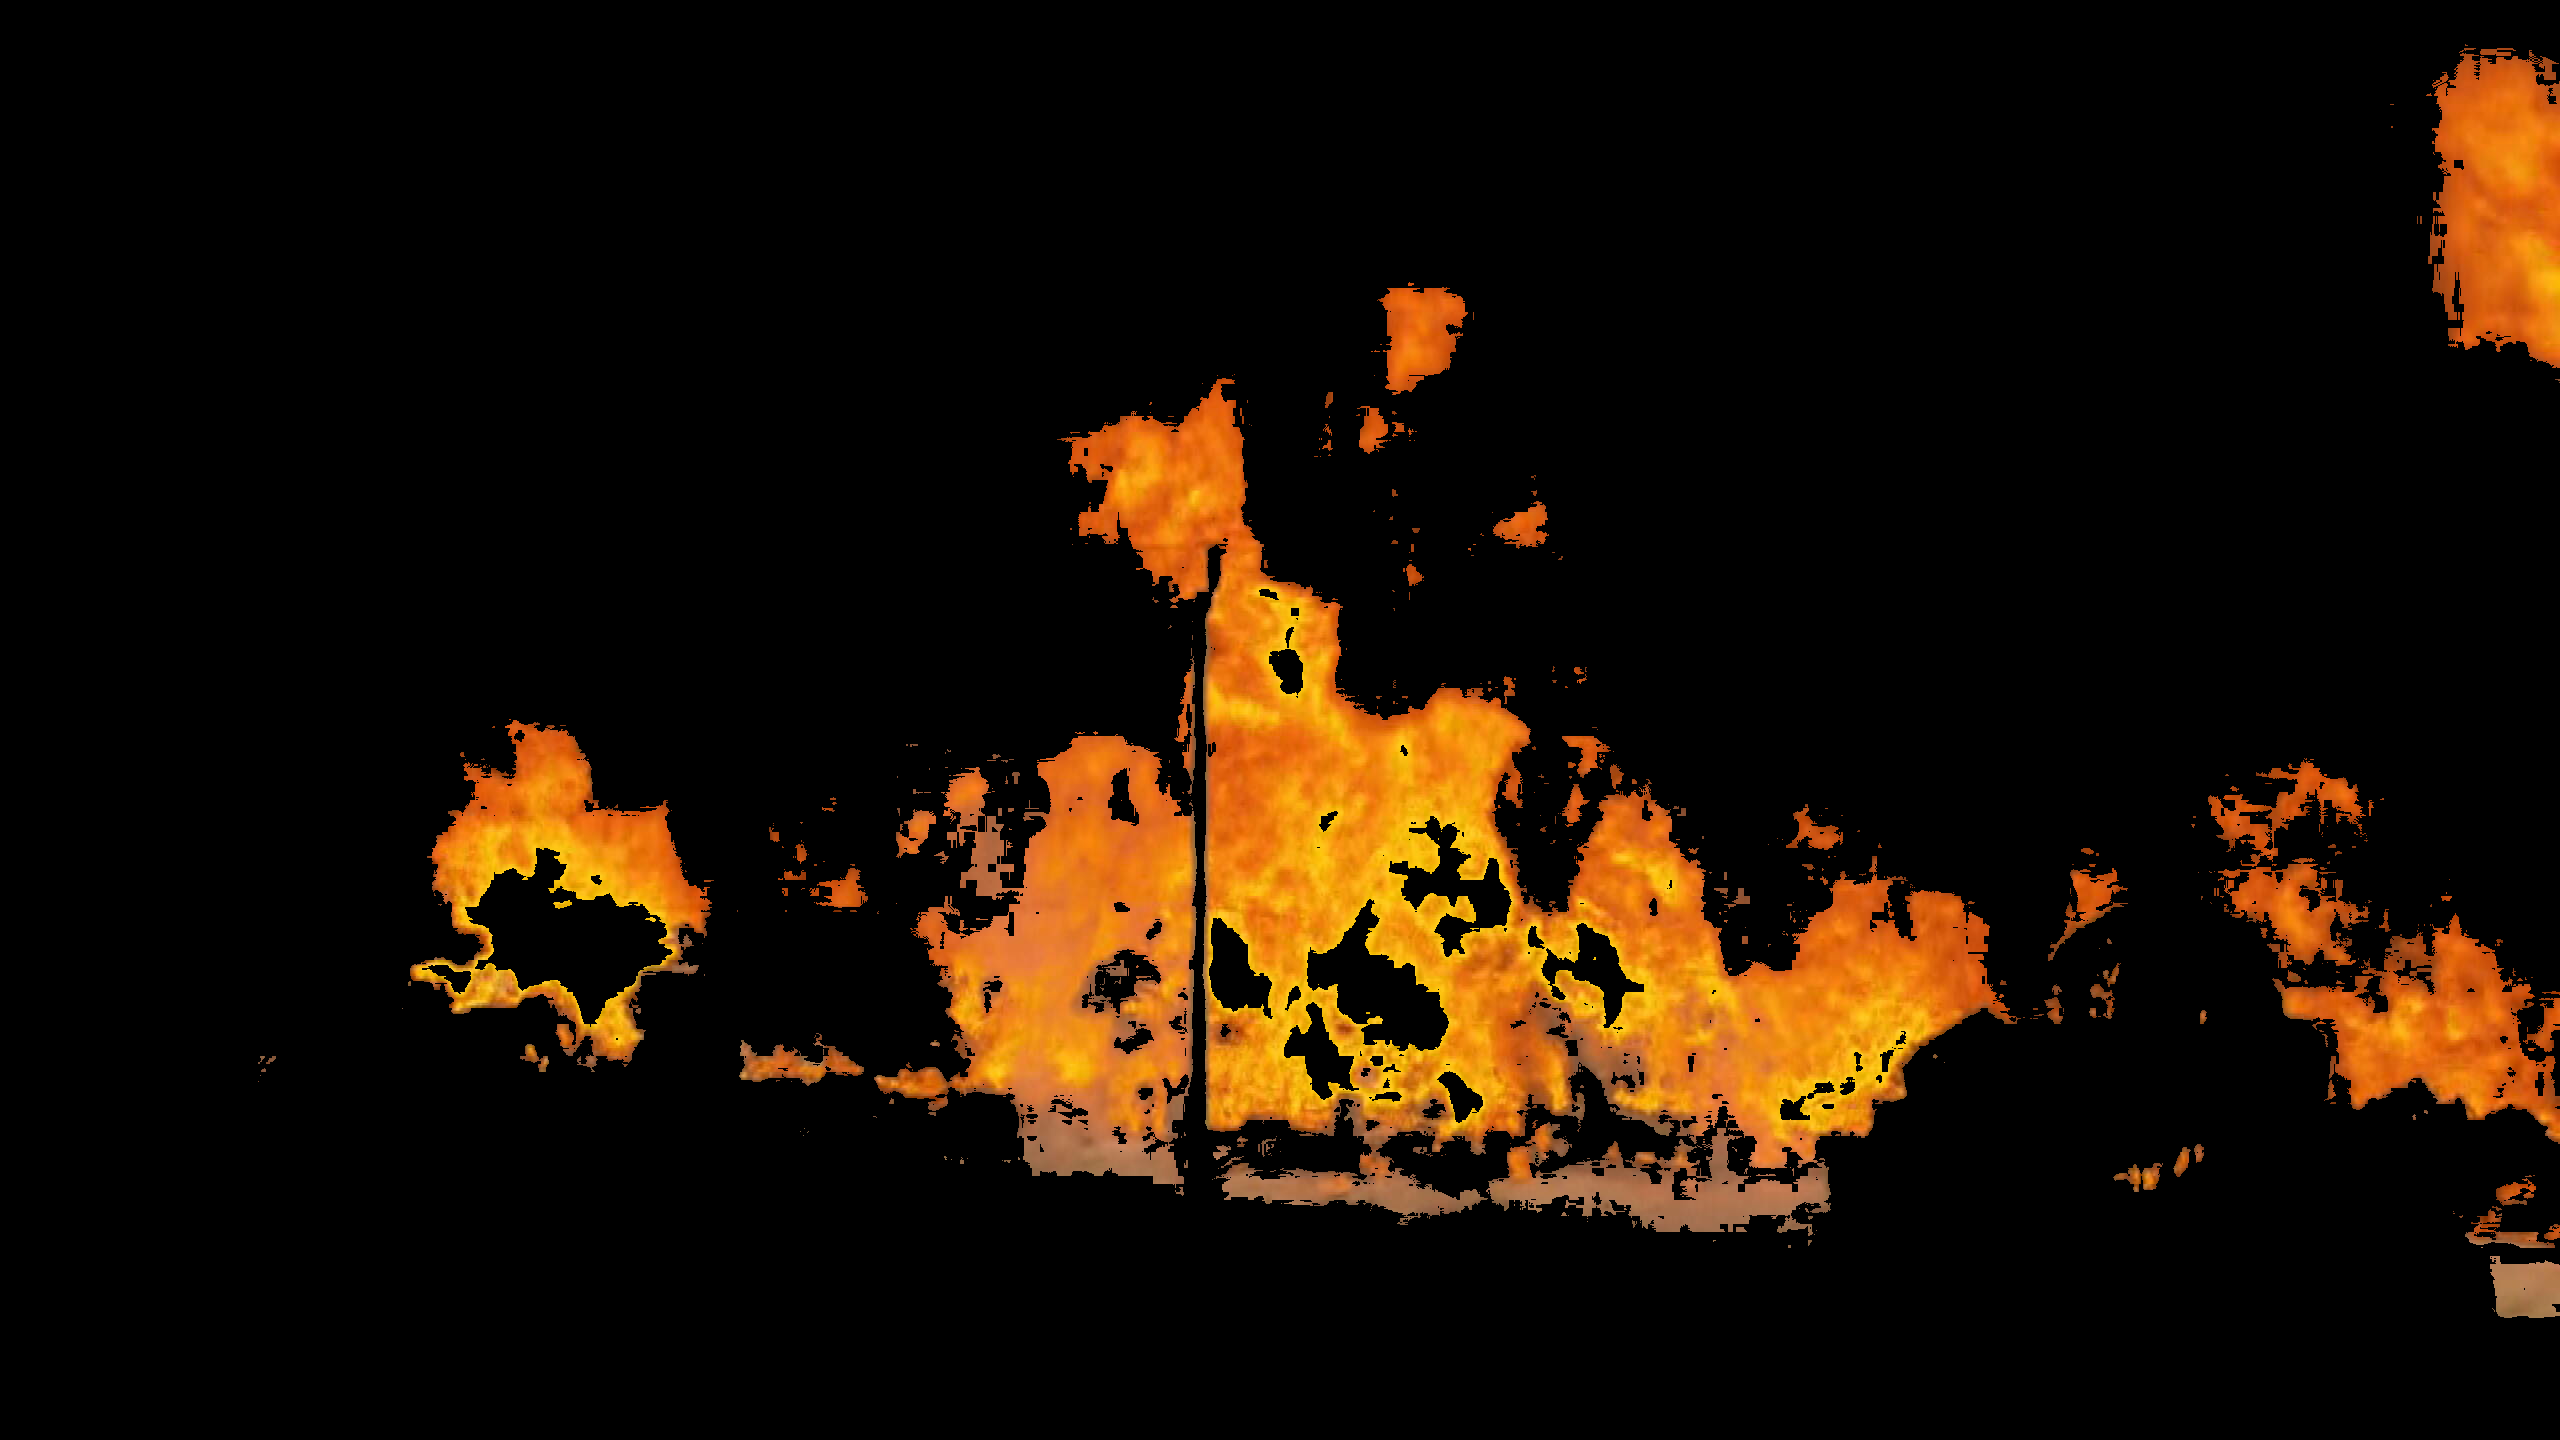
\includegraphics[width=\textwidth]{hsv_filter.png}
%                 \caption{$filtered image$}
%                 \label{fig:y equals x}
%         \end{subfigure}
%         \hfill
%         \begin{subfigure}[b]{0.5\textwidth}
%                 \centering
%                 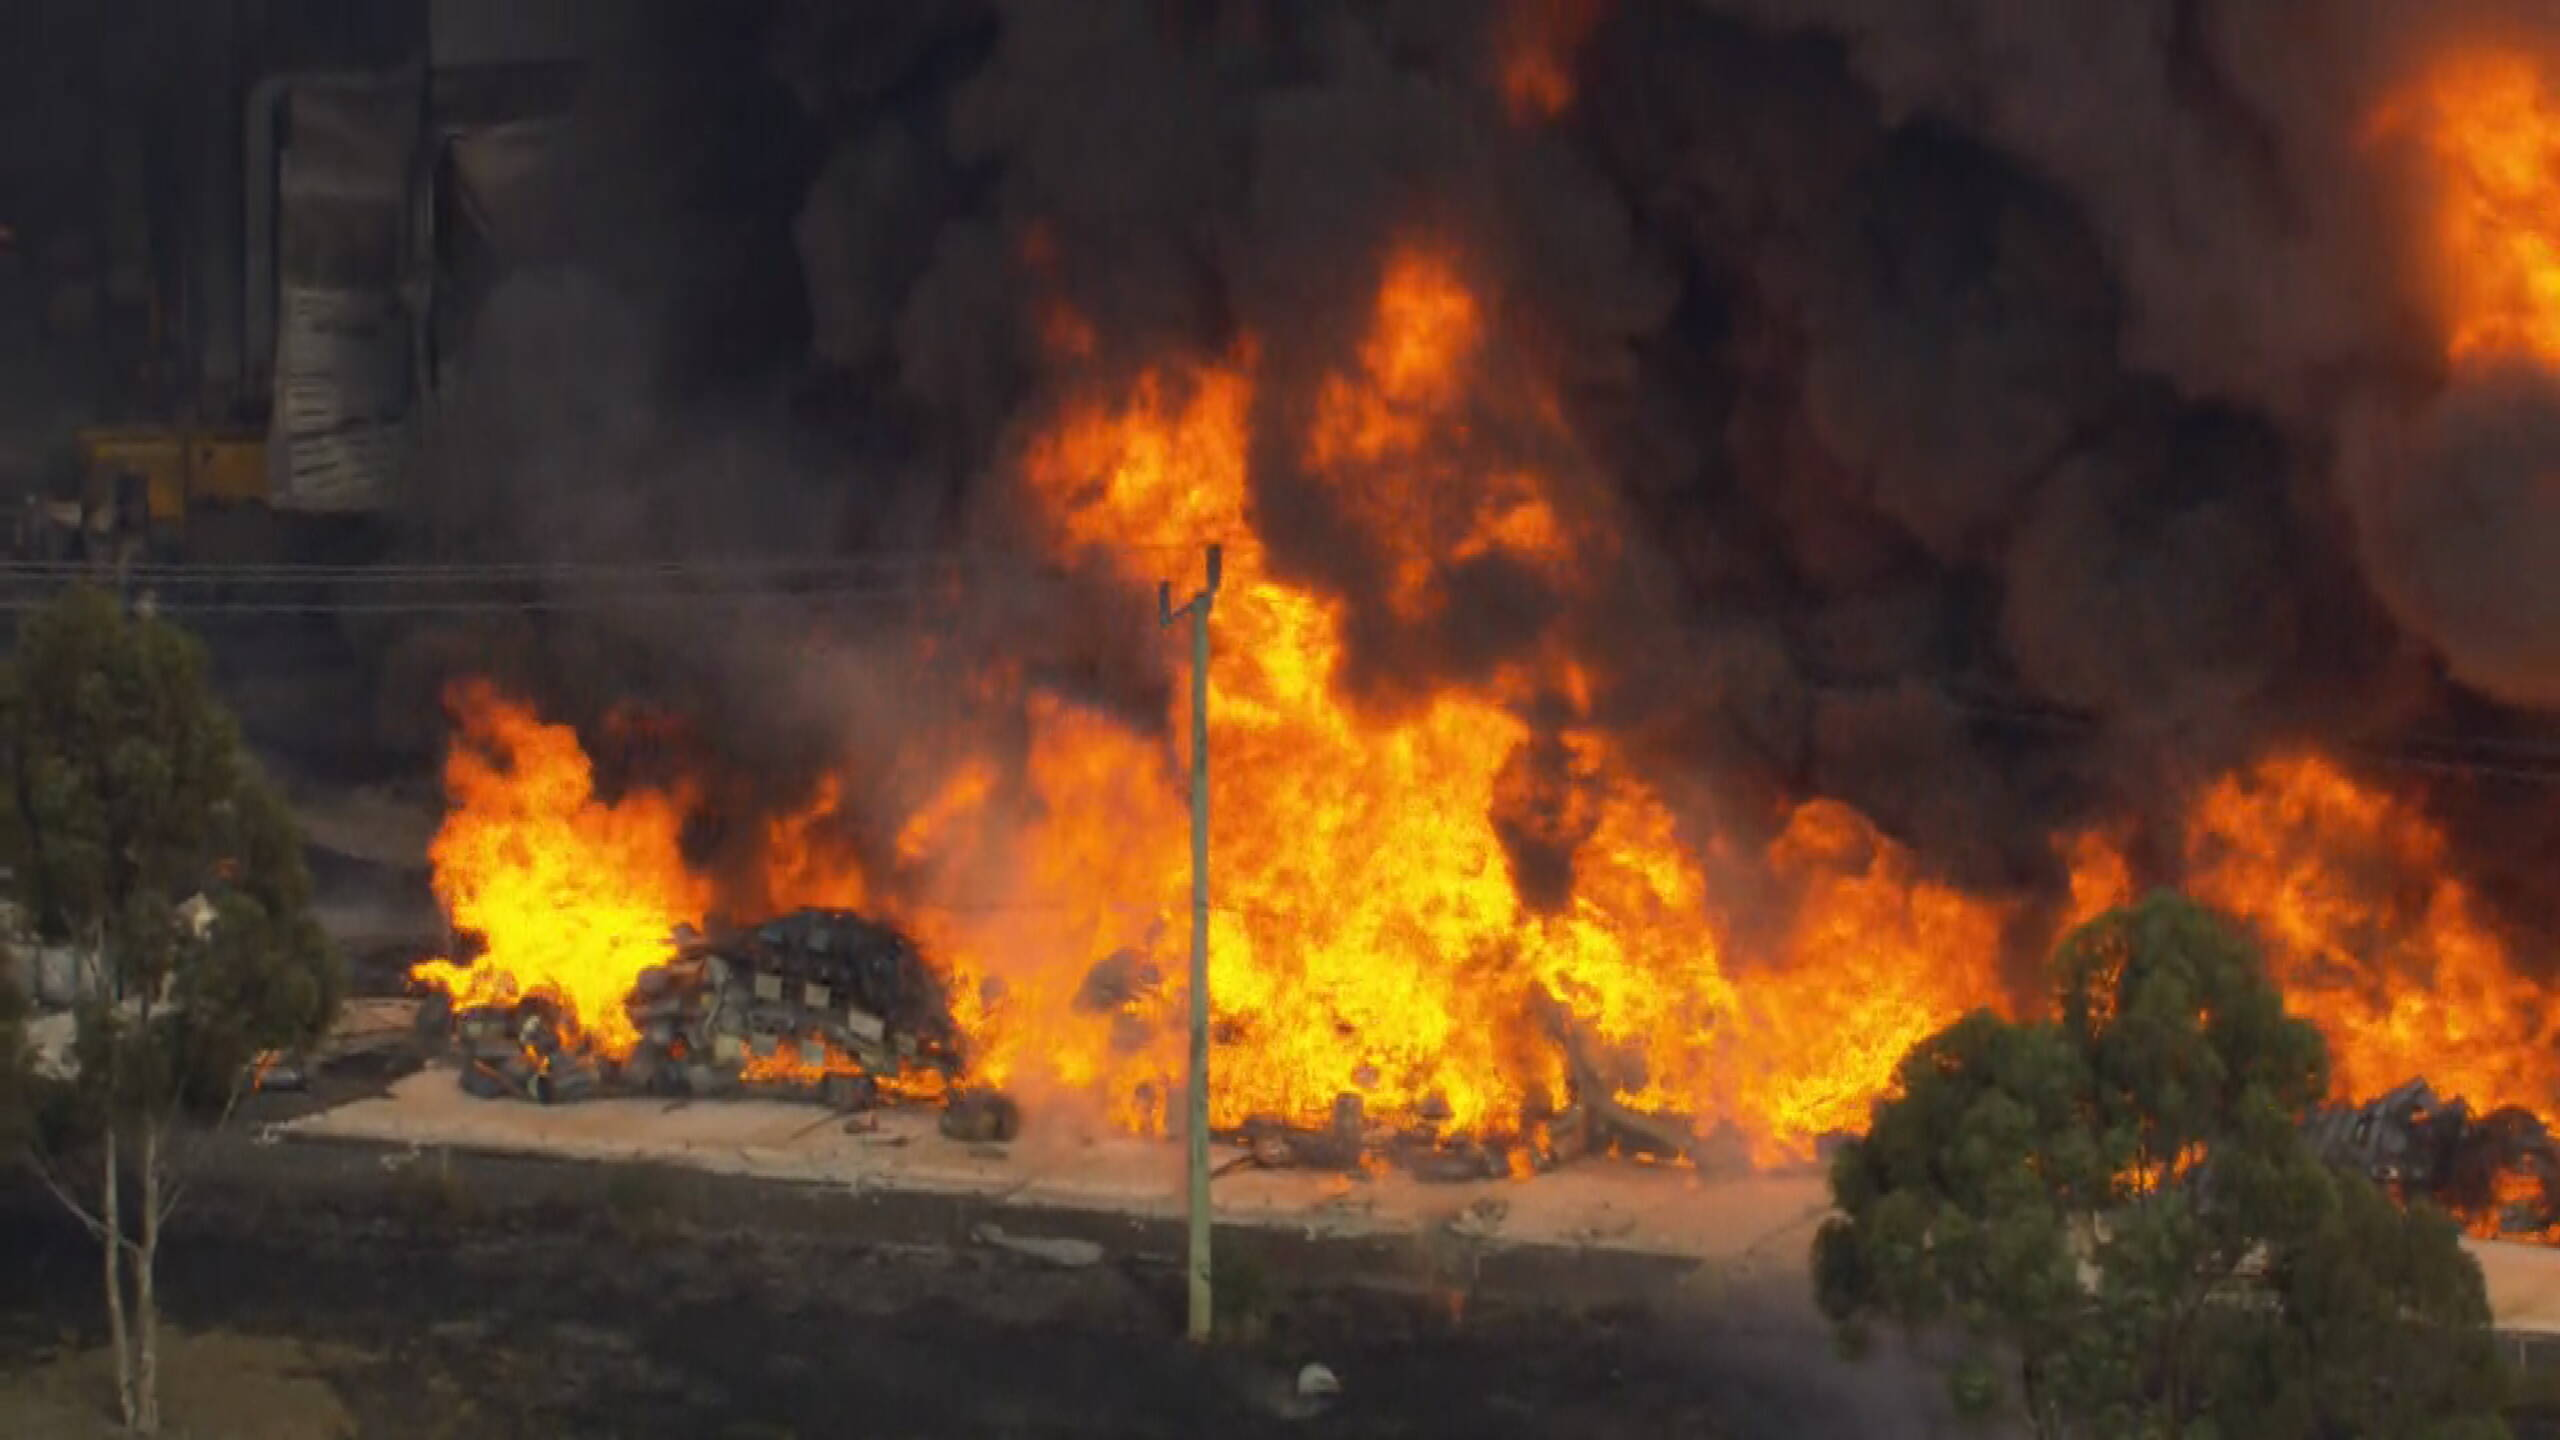
\includegraphics[width=\textwidth]{hsv_original.jpeg}
%                 \caption{$original image$}
%                 \label{fig:y equals x}
%         \end{subfigure}
%         \caption{Resulting Image after HSV mask}
% \end{figure}

\begin{figure*}[!t]
\centering
\subfloat[]{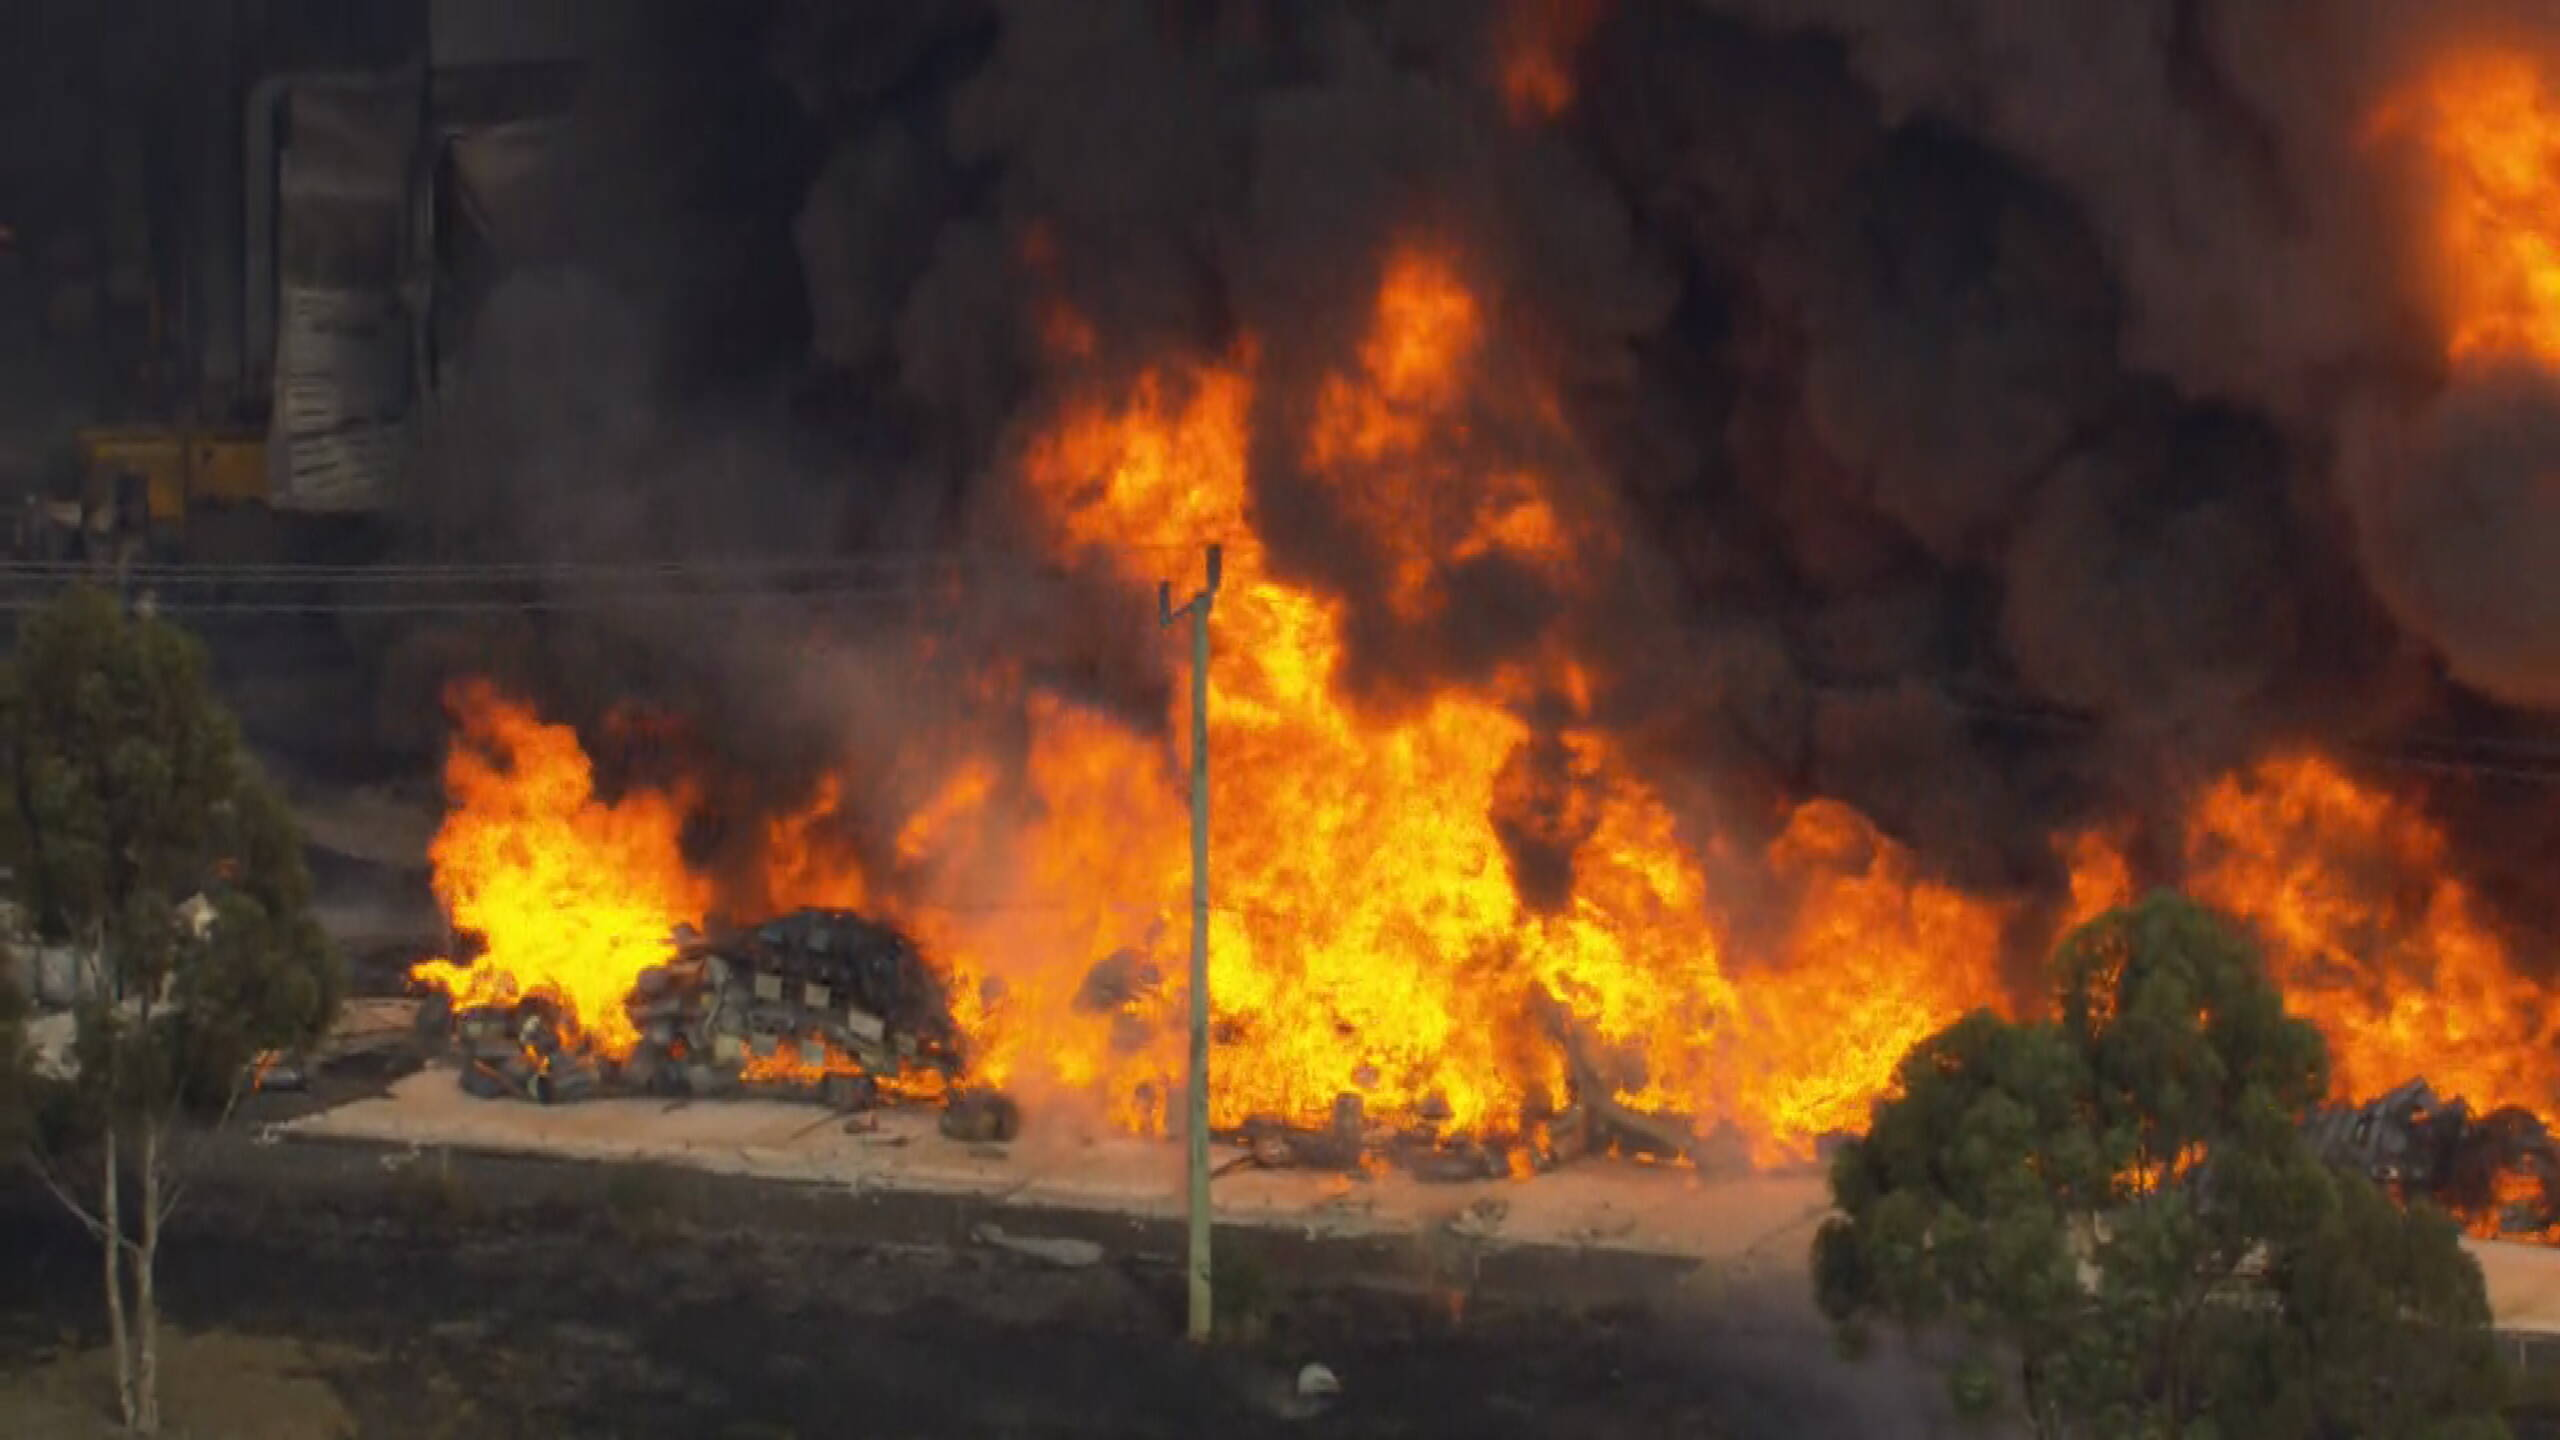
\includegraphics[width=2.5in]{hsv_original.jpeg}%
\label{hsv_orig}}
\hfil
\subfloat[]{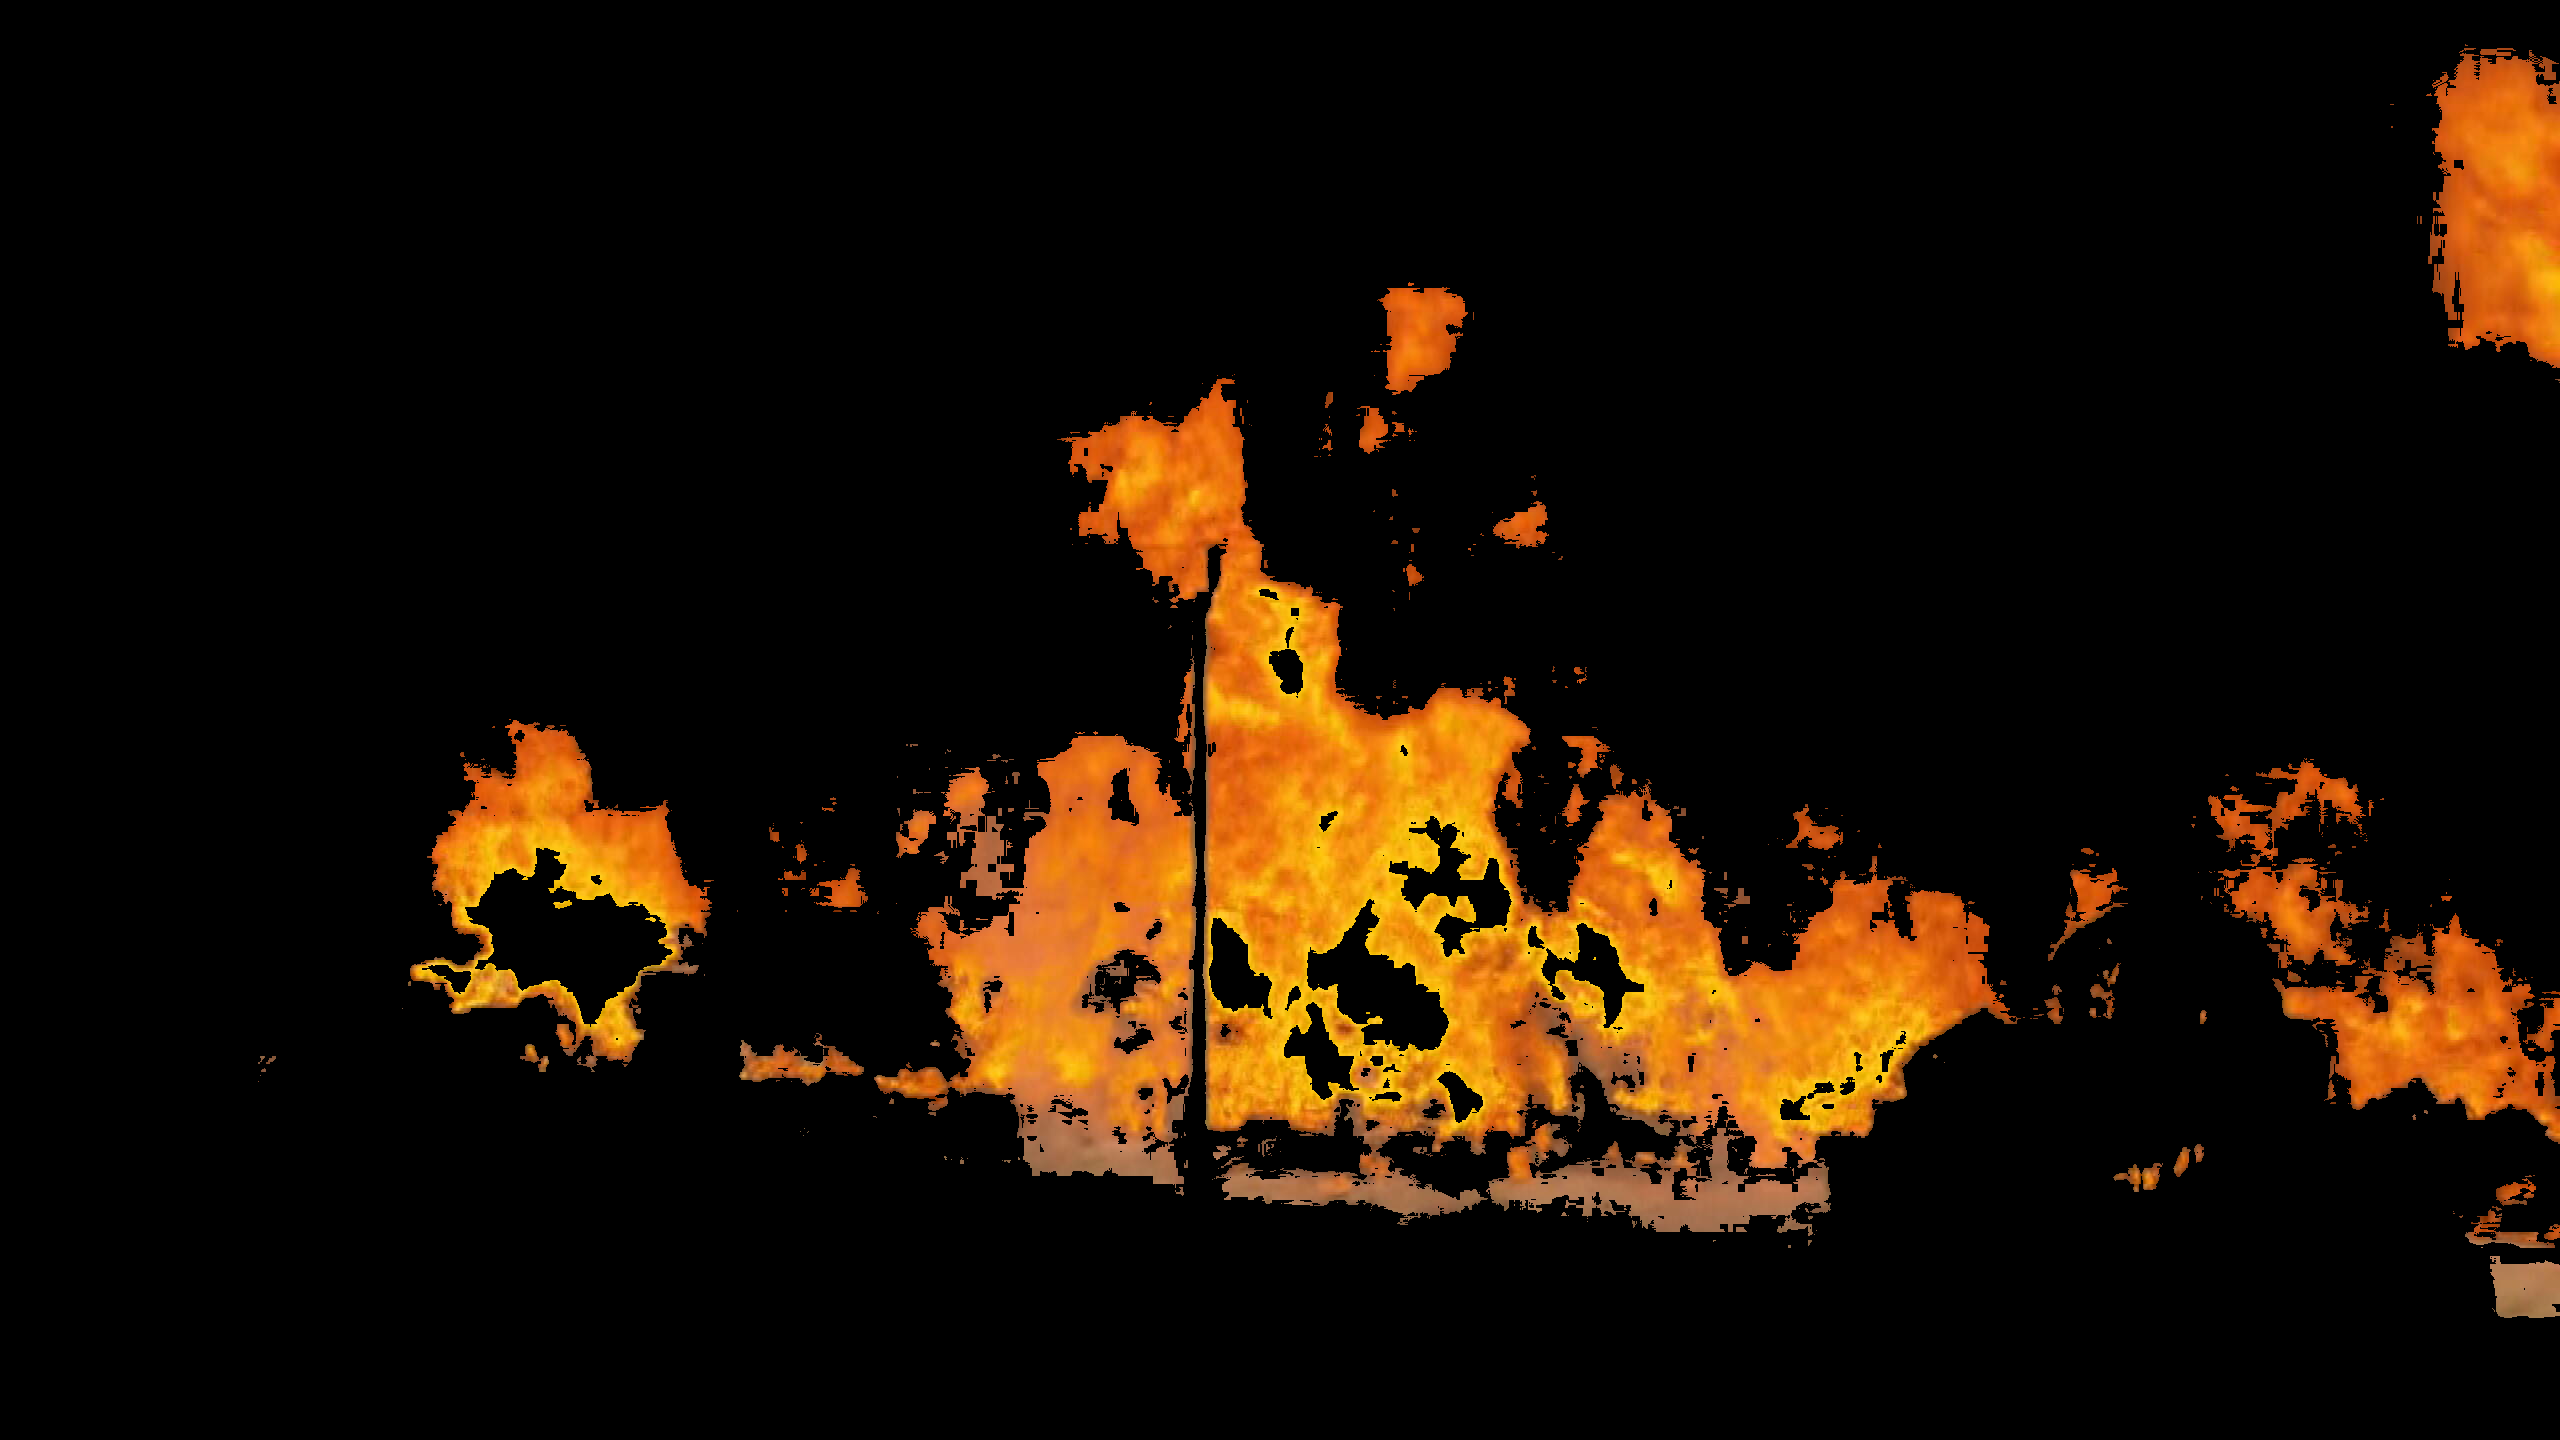
\includegraphics[width=2.5in]{hsv_filter.png}%
\label{hsv_filter}}
        \caption{Example of Image filtered using the described HSV mask. (a) Original image. (b) Filtered image.}
\label{hsvimg}
\end{figure*}

\subsection{Automatic Annotation}

High quality annotated training data is crucial for creating a performant segmentation model. However, manually annotating images requires substantial human effort. As a result, automatic annotation methods have emerged, leveraging pre-trained detection along with prompt based segmentation models to significantly reduce human workload. 

\bibliographystyle{IEEEtran}
\bibliography{ref}

\newpage


\vfill

\end{document}


